%%This is a very basic article template.
%%There is just one section and two subsections.
\documentclass{article}
\usepackage[utf8]{inputenc}              	%nastaven� v�choz�ho k�dov�n� textu
\usepackage[czech]{babel}                	%nastaven� �esk�ch znak�
\usepackage[pdftex]{graphicx}				%umo��uje vkl�d�n� obr�zk� v jpg, png
\usepackage{amsfonts}						%package obsahujici symboly mnozin treba - \mathbb{N}
%\usepackage{amssymb}						%stejna funkce jako amsfonts				%stejna funkce jako amsfonts
\usepackage[square, numbers]{natbib} 		%sazba pouzite literatury, bibliography

\begin{document}
\section{Validátory}
Vzhledem k některým guardům, které nemapují entity, pokud je model v
nekonzistentním stavu jsme se rozhodli pro vytvoření validačního query, které
zkontroluje stav modelu. Toto query se dá použít na vstupní  i výstupní model.

\section{Validátor aplikačního modelu}
Nekonzistentní stavy modelu se dělí do těchto kategorií:
\begin{itemize}
  \item duplicitní jména(Class, property, \ldots)
  \item hierarchie dědičnosti
  \item primitivní typy
  \item vazby
  \item embeddedClass
\end{itemize}

\subsection{Duplicitní jména}
Neexistuje Class v generaci se jménem shodným s jménem jiné třídy v téže
generaci \newline

Neexistuje property ve třídě se shodným jménem s property téže třídy nebo jejího
předka - zamezujeme překrývání vyobrazeném na obrázku
\ref{pict:prekryvani_atributu}, ackoliv toto je v Jave mozne.

\begin{figure}[th]
	\begin{center}
	\refstepcounter{figure}
	\label{pict:prekryvani_atributu}		             
    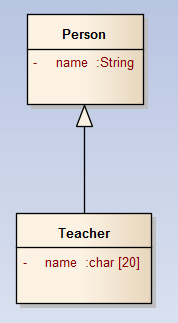
\includegraphics[scale=1.0]{../images/prekryvani_atributu.png}
	\caption{Překrývání atributů tříd}
	\end{center}			     
\end{figure}


\subsection{hierarchie ddičnosti}
Neexistuje třída, která by sobě samé byla předkem ( v hierarchii nevzniká
cyklus)

Trida je embedded nebo je primitive nebo ma parenta nebo ma prave jednu property
s atributem isID nastavenym na true.

\subsection{Primitivní tridy}
Neexistuje primitivní třída, která by měla id

\subsection{Property + vazby}
%%to chce prepsat
Neexistuje třída, která by měla property neprimitivního typu, jejíž opposite
property by nebyla nastavená původní property. 
Všechny primitivní Property mají nastavenou oppositeProperty na null 

Neexistuje property nelistové třídy (nelistová třída = třída mající potomka)
mapovanýma přes InheritanceType TablePerClass a upperBound vyšší než 1.

Neexistuje primitivní property s arritou 1..N , kde N > 1, která by měla stejné
jméno jako nějaká třída v generaci. Pozn. jde o mapování kolekcí, které potřebují
vlastní tabulku.

%%% Neexistuje property s lowerBound jinou než 0 nebo 1.

\subsection{EmbeddedClass}
Neexistuje embeddedClass v generaci, která by měla property jiné arrity než
0 \ldots 1 x 1 nebo 1 x 1 \newline

V rámci třídy neexistuje Property v hierarchii, která by měla name shodné s
Stringem reprezentujícím property typu EmbeddedTřída. Poznámka: reprezentativní
Stringy property se rovnají:\newline
 property.name + "\_" + property.type.property[i].name \newline

Na obr. \ref{pict:embedded-collision} vidíme příklad takové kolize jmen.
Reprezentativními Stringy jsou "income\_amount" a "income\_currency", které jsou
v kolizi s jménem property třídy Person. Druhou chybou je multiplicita M x N.
\begin{figure}[t]
	\begin{center}
	\refstepcounter{figure}
	\label{pict:embedded-collision}		             
    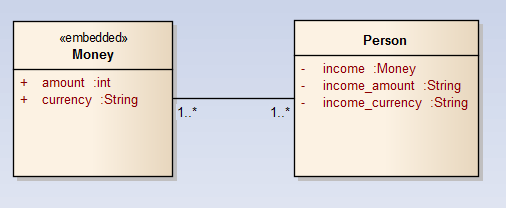
\includegraphics[scale=1.0]{../images/embedded_collision_example.png}
	\caption{EmbeddedClass kolize}
	\end{center}			     
\end{figure}


\section{Validator DB modelu}
\subsection {Case Sentivity} SQL není case sensitive jazyk, takže kolize jmen v
DB modelu nastává i v případě neshodných identifikátorů např. "lambda" a
"LaMBDA". Nynější implementace povoluje vytvoření modelu s velkými i malými
písmeny.
\subsection{Identifikátory}
Podle dokumentace PostgreSQL viz \cite{www:postgreSQL:identifiers} a
\cite{www:postgreSQL:keywords} každý SQL identifikátor v postgreSQL je může
obsahovat písmena (a-z), pomlčku \_, diakritické znaky, písmena jiné než
latinské abecedy, číslice, symbol dolar(\#) nebo podtržíteka. Dále pak každý
identifikátor musí začínat jedním z písmen (a-z) a nesmí být rezervované
klíčové slovo či nerezervované slovo v kontextu.

Pro zjednodušení jsme si určili, že každý identifikátor musí začínat písmeny
"(a-z)" a kromě těchto písmen může dále pak obsahovat pomlčku (\_) a
latinské číslice. \\


Model není validní, pokud není některý vygenerovaný identifikátor validní.\\

Model není validní, pokud identifikátor koliduje s klíčovým SQL slovem z
následujícího seznamu


ABORT,
ABSOLUTE,
ACCESS,
ACTION,
ADD,
ADMIN,
AFTER,
AGGREGATE,
ALL,
ALSO,
ALTER,
ALWAYS,
ANALYSE,
ANALYZE,
AND,
ANY,
ARRAY,
AS,
ASC,
ASSERTION,
ASSIGNMENT,
ASYMMETRIC,
AT,
AUTHORIZATION,
BACKWARD,
BEFORE,
BEGIN,
BETWEEN,
BIGINT,
BINARY,
BIT,
BOOLEAN,
BOTH,
BY,
CACHE,
CALLED,
CASCADE,
CASCADED,
CASE,
CAST,
CATALOG,
CHAIN,
CHAR,
CHARACTER,
CHARACTERISTICS,
CHECK,
CHECKPOINT,
CLASS,
CLOSE,
CLUSTER,
COALESCE,
COLLATE,
COLUMN,
COMMENT,
COMMENTS,
COMMIT,
COMMITTED,
CONCURRENTLY,
CONFIGURATION,
CONNECTION,
CONSTRAINT,
CONSTRAINTS,
CONTENT,
CONTINUE,
CONVERSION,
COPY,
COST,
CREATE,
CREATEDB,
CREATEROLE,
CREATEUSER,
CROSS,
CSV,
CURRENT,
CURRENT\_CATALOG,
CURRENT\_DATE,
CURRENT\_ROLE,
CURRENT\_SCHEMA,
CURRENT\_TIME,
CURRENT\_TIMESTAMP,
CURRENT\_USER,
CURSOR,
CYCLE,
DATA,
DATABASE,
DAY,
DEALLOCATE,
DEC,
DECIMAL,
DECLARE,
DEFAULT,
DEFAULTS,
DEFERRABLE,
DEFERRED,
DEFINER,
DELETE,
DELIMITER,
DELIMITERS,
DESC,
DICTIONARY,
DISABLE,
DISCARD,
DISTINCT,
DO,
DOCUMENT,
DOMAIN,
DOUBLE,
DROP,
EACH,
ELSE,
ENABLE,
ENCODING,
ENCRYPTED,
END,
ENUM,
ESCAPE,
EXCEPT,
EXCLUDE,
EXCLUDING,
EXCLUSIVE,
EXECUTE,
EXISTS,
EXPLAIN,
EXTERNAL,
EXTRACT,
FALSE,
FAMILY,
FETCH,
FIRST,
FLOAT,
FOLLOWING,
FOR,
FORCE,
FOREIGN,
FORWARD,
FREEZE,
FROM,
FULL,
FUNCTION,
FUNCTIONS,
GLOBAL,
GRANT,
GRANTED,
GREATEST,
GROUP,
HANDLER,
HAVING,
HEADER,
HOLD,
HOUR,
IDENTITY,
IF,
ILIKE,
IMMEDIATE,
IMMUTABLE,
IMPLICIT,
IN,
INCLUDING,
INCREMENT,
INDEX,
INDEXES,
INHERIT,
INHERITS,
INITIALLY,
INLINE,
INNER,
INOUT,
INPUT,
INSENSITIVE,
INSERT,
INSTEAD,
INT,
INTEGER,
INTERSECT,
INTERVAL,
INTO,
INVOKER,
IS,
ISNULL,
ISOLATION,
JOIN,
KEY,
LANGUAGE,
LARGE,
LAST,
LC\_COLLATE,
LC\_CTYPE,
LEADING,
LEAST,
LEFT,
LEVEL,
LIKE,
LIMIT,
LISTEN,
LOAD,
LOCAL,
LOCALTIME,
LOCALTIMESTAMP,
LOCATION,
LOCK,
LOGIN,
MAPPING,
MATCH,
MAXVALUE,
MINUTE,
MINVALUE,
MODE,
MONTH,
MOVE,
NAME,
NAMES,
NATIONAL,
NATURAL,
NCHAR,
NEXT,
NO,
NOCREATEDB,
NOCREATEROLE,
NOCREATEUSER,
NOINHERIT,
NOLOGIN,
NONE,
NOSUPERUSER,
NOT,
NOTHING,
NOTIFY,
NOTNULL,
NOWAIT,
NULL,
NULLIF,
NULLS,
NUMERIC,
OBJECT,
OF,
OFF,
OFFSET,
OIDS,
ON,
ONLY,
OPERATOR,
OPTION,
OPTIONS,
OR,
ORDER,
OUT,
OUTER,
OVER,
OVERLAPS,
OVERLAY,
OWNED,
OWNER,
PARSER,
PARTIAL,
PARTITION,
PASSWORD,
PLACING,
PLANS,
POSITION,
PRECEDING,
PRECISION,
PREPARE,
PREPARED,
PRESERVE,
PRIMARY,
PRIOR,
PRIVILEGES,
PROCEDURAL,
PROCEDURE,
QUOTE,
RANGE,
READ,
REAL,
REASSIGN,
RECHECK,
RECURSIVE,
REFERENCES,
REINDEX,
RELATIVE,
RELEASE,
RENAME,
REPEATABLE,
REPLACE,
REPLICA,
RESET,
RESTART,
RESTRICT,
RETURNING,
RETURNS,
REVOKE,
RIGHT,
ROLE,
ROLLBACK,
ROW,
ROWS,
RULE,
SAVEPOINT,
SCHEMA,
SCROLL,
SEARCH,
SECOND,
SECURITY,
SELECT,
SEQUENCE,
SEQUENCES,
SERIALIZABLE,
SERVER,
SESSION,
SESSION\_USER,
SET,
SETOF,
SHARE,
SHOW,
SIMILAR,
SIMPLE,
SMALLINT,
SOME,
STABLE,
STANDALONE,
START,
STATEMENT,
STATISTICS,
STDIN,
STDOUT,
STORAGE,
STRICT,
STRIP,
SUBSTRING,
SUPERUSER,
SYMMETRIC,
SYSID,
SYSTEM,
TABLE,
TABLES,
TABLESPACE,
TEMP,
TEMPLATE,
TEMPORARY,
TEXT,
THEN,
TIME,
TIMESTAMP,
TO,
TRAILING,
TRANSACTION,
TREAT,
TRIGGER,
TRIM,
TRUE,
TRUNCATE,
TRUSTED,
TYPE,
UNBOUNDED,
UNCOMMITTED,
UNENCRYPTED,
UNION,
UNIQUE,
UNKNOWN,
UNLISTEN,
UNTIL,
UPDATE,
USER,
USING,
VACUUM,
VALID,
VALIDATOR,
VALUE,
VALUES,
VARCHAR,
VARIADIC,
VARYING,
VERBOSE,
VERSION,
VIEW,
VOLATILE,
WHEN,
WHERE,
WHITESPACE,
WINDOW,
WITH,
WITHOUT,
WORK,
WRAPPER,
WRITE,
XML,
XMLATTRIBUTES,
XMLCONCAT,
XMLELEMENT,
XMLFOREST,
XMLPARSE,
XMLPI,
XMLROOT,
XMLSERIALIZE,
YEAR,
YES,
ZONE \\

\bibliographystyle{plainnat}
\bibliography{references}
\end{document}
